\documentclass[proposal,indonesia]{ugmskripsi}
% Options:
%   skripsi / proposal        (default: skripsi)
%   satuspasi / duaspasi / satusetengahspasi (default: satusetengahspasi)
%   indonesia / inggris       (default: indonesia)

%------------------------------------------------------------
% Metadata Proposal
%------------------------------------------------------------
% Metadata penulis
\titleind{Sequence-Level Routing untuk Efisiensi Inferensi Qwen3-0.6B pada Peringkasan Berita Bahasa Indonesia}
\titleeng{Sequence-Level Routing for Efficient Qwen3-0.6B Inference in Indonesian News Summarization}
\fullname{Joseph Greffen Komala}
\idnum{23/519909/PA/22318}
\degree{JENJANG}
\gelar{GELAR}
\yearsubmit{TAHUN}
\program{[ISI NAMA PROGRAM STUDI]}
\dept{[ISI NAMA DEPARTEMEN]}
\firstsupervisor{NAMA DOSEN PEMBIMBING}
\firstexaminer{NAMA DOSEN PENGUJI 1}
\secondexaminer{NAMA DOSEN PENGUJI 2}
\examdate{TANGGAL UJIAN BELUM DITETAPKAN}

%------------------------------------------------------------
% Packages
%------------------------------------------------------------
\usepackage[utf8]{inputenc}
\usepackage{graphicx}
\graphicspath{{figures/}}
\usepackage{amsmath}
\usepackage{amssymb}
\usepackage{booktabs}
\usepackage{longtable}
\usepackage{tabularx}
\usepackage{multirow}
\usepackage{float}
\usepackage{listings}
\usepackage{xcolor}
\usepackage{hyperref}
\hypersetup{hidelinks}
\usepackage{url}
\usepackage{enumitem}
\usepackage{tikz}
\usetikzlibrary{arrows.meta,positioning}
\setlength{\emergencystretch}{3em}

% Code listing style
\lstset{
    basicstyle=\ttfamily\small,
    breaklines=true,
    frame=single,
    numbers=left,
    numberstyle=\tiny,
    keywordstyle=\color{blue},
    commentstyle=\color{gray},
    stringstyle=\color{orange},
    showstringspaces=false,
    tabsize=2
}

% Define YAML language for listings
\lstdefinelanguage{yaml}{
  keywords={true,false,null,y,n},
  sensitive=false,
  comment=[l]{\#},
  morecomment=[s]{/*}{*/},
  morestring=[b]',
  morestring=[b]"
}

% Define Docker language for listings
\lstdefinelanguage{docker}{
  alsoletter={-},
  keywords={FROM,RUN,CMD,LABEL,MAINTAINER,EXPOSE,ENV,ADD,COPY,ENTRYPOINT,VOLUME,USER,WORKDIR,ARG,ONBUILD,STOPSIGNAL,HEALTHCHECK,SHELL},
  sensitive=false,
  comment=[l]{\#},
  morestring=[b]',
  morestring=[b]"
}

%------------------------------------------------------------
% Document Body
%------------------------------------------------------------
\begin{document}

% Preliminary Pages (Proposal: minimal)
\begingroup
\setkeys{Gin}{width=5.5cm}
\cover
\clearpage
\titlepageind
\clearpage
\endgroup
\begingroup
\setlength{\tabcolsep}{0pt}
\approvalpage
\clearpage
\endgroup

\tableofcontents

\abstractind

Penelitian ini akan mengukur hubungan antara kualitas ringkasan dan efisiensi inferensi Qwen3-0.6B pada tugas peringkasan berita bahasa Indonesia menggunakan XL-Sum subset Indonesia. Mekanisme yang dikaji adalah pemilihan jalur eksekusi satu kali untuk setiap urutan masukan dan keluaran (\textit{sequence-level routing}). Dari 28 lapisan model, lima kelompok tengah dapat dijalankan atau dilewati; kelompok pertama dan terakhir selalu dijalankan. Sebuah router menggunakan rata-rata vektor representasi internal token artikel setelah kelompok pertama untuk menentukan keputusan tersebut. Keputusan yang sama dipakai selama sisa pemrosesan prompt dan seluruh pembentukan token keluaran. Pelatihan dilakukan dalam dua tahap: router dilatih saat parameter Qwen dibekukan, kemudian router dibekukan dan adapter \textit{Low-Rank Adaptation} (LoRA) dilatih untuk mengompensasi dampak pelompatan lapisan. Target router dibuat dari pencarian bertahap yang membandingkan kerugian prediksi token dengan proporsi kelompok lapisan yang aktif. Evaluasi membandingkan model penuh, pelompatan statis, dan routing adaptif dengan pelatihan LoRA yang setara, serta router tanpa LoRA sebagai kontrol. Kualitas dinilai secara otomatis menggunakan skor F1 pada ROUGE-1, ROUGE-2, ROUGE-L, dan BERTScore. Skor F1 dihitung per artikel, dirata-ratakan secara terpisah untuk setiap metrik, lalu dilaporkan tanpa digabung menjadi satu skor. Efisiensi dinilai dari waktu total per artikel, termasuk biaya router, waktu pemrosesan prompt, waktu pembentukan keluaran, dan jumlah token keluaran. Penelitian ini tidak mengasumsikan bahwa routing akan unggul. Eksperimen menggunakan 1.000 artikel latih, 200 artikel validasi, dan 300 artikel uji pada laptop lokal; penelitian direncanakan berlangsung selama empat bulan.
\endabstractind

\abstracteng

This study will measure the relationship between summary quality and inference efficiency for Qwen3-0.6B on Indonesian news summarization using the Indonesian subset of XL-Sum. It will examine sequence-level routing, which selects an execution path once for each input-and-output sequence. The model's 28 layers will be divided into seven consecutive groups of four. The first and last groups will always run, while a router will decide whether to run or skip each of the five middle groups. The router will use the mean internal representation of article tokens after the first group, and its decisions will remain fixed for the rest of prompt processing and all output-token generation. Training will use two stages: first, train the router while Qwen remains frozen; then freeze the router and train Low-Rank Adaptation (LoRA) adapters to compensate for layer skipping. Router targets will be produced by a greedy search balancing teacher-forced token prediction loss against the proportion of active middle groups. Evaluation will compare full-model, static-skipping, and adaptive-routing variants trained with LoRA, as well as routing without LoRA as a control. Quality will be assessed automatically using ROUGE-1, ROUGE-2, ROUGE-L, and BERTScore F1, calculated per article and averaged separately for each metric. Efficiency measures will include total time per article, router overhead, prompt-processing time, output-generation time, and output length. The study will not assume that routing will outperform the alternatives. The experiment will use 1,000 training articles, 200 validation articles, and 300 test articles on the local laptop; the study is planned to last four months.
\endabstracteng

%------------------------------------------------------------
% Chapters
%------------------------------------------------------------
\chapter{PENDAHULUAN}

\section{Latar Belakang}

Model bahasa menghasilkan teks sedikit demi sedikit dalam satuan yang disebut token (potongan teks). Pada setiap langkah inferensi, yaitu saat model digunakan untuk menghasilkan keluaran, model menghitung representasi melalui lapisan-lapisan Transformer, sebuah arsitektur jaringan saraf, sebelum memilih token berikutnya. Penghitungan berulang ini dapat membuat proses inferensi memerlukan waktu dan komputasi yang besar. FiRST, misalnya, mengkaji pengurangan waktu inferensi dengan melewati sebagian lapisan berdasarkan masukan \citep{jain2025first}. Namun, pengurangan komputasi perlu dinilai bersama perubahan kualitas teks yang dihasilkan.

Salah satu cara mengurangi penghitungan tersebut adalah \textit{layer skipping}, yaitu melewati lapisan tertentu saat model menghasilkan keluaran. Pada strategi statis, lapisan yang dijalankan sama untuk semua masukan. Pada strategi adaptif, keputusan lapisan dapat bergantung pada isi masukan. PuDDing menggunakan router, yaitu komponen ringan yang memilih lapisan untuk dijalankan, berdasarkan prompt (teks masukan yang berisi instruksi dan bahan untuk diproses) \citep{wee2025pudding}. Hasil PuDDing pada tugas penalaran akal sehat yang diuji dalam penelitian tersebut menjadi bukti bagi pendekatan pemilihan adaptif pada tugas-tugas itu, tetapi tidak memastikan hasil yang sama pada peringkasan berita bahasa Indonesia.

Penelitian ini mengkaji pemilihan jalur eksekusi pada tingkat urutan masukan dan keluaran (\textit{sequence-level routing}). Router membaca representasi artikel satu kali untuk menentukan apakah setiap kelompok lapisan tengah dijalankan atau dilewati. Keputusan yang sama dipertahankan selama sisa pemrosesan prompt dan seluruh pembentukan token keluaran (\textit{decoding}), sehingga jalur tidak dipilih ulang pada setiap token. Pelatihan dilakukan dalam dua tahap, mengikuti pola yang digunakan FiRST \citep{jain2025first}. Pada tahap pertama, parameter model utama dibekukan dan hanya router yang dilatih. Pada tahap kedua, router dibekukan dan adapter Low-Rank Adaptation (LoRA) dilatih pada modul attention dan FFN untuk mengompensasi dampak pelompatan lapisan. Target router dibentuk dari ringkasan acuan dengan membandingkan kerugian prediksi token untuk sejumlah pola kelompok lapisan.

Model utama (\textit{backbone}) yang digunakan adalah Qwen3-0.6B, yaitu model bahasa kausal yang memprediksi token berikutnya berdasarkan teks sebelumnya, dengan ukuran nominal 0,6 miliar parameter dan 28 lapisan \citep{qwen2025modelcard}. Tugas penelitian adalah peringkasan berita bahasa Indonesia menggunakan bagian berbahasa Indonesia dari XL-Sum. Dataset XL-Sum berisi pasangan artikel dan ringkasan yang disiapkan untuk penelitian peringkasan abstraktif, yaitu peringkasan yang merumuskan kembali informasi penting dengan kalimat baru \citep{hasan2021xlsum}. Ringkasan acuan digunakan saat membentuk target pelatihan router, tetapi tidak diberikan kepada router sebagai masukan saat inferensi.

Jumlah lapisan yang dilewati saja belum menunjukkan manfaat praktis. Router menambah pekerjaan komputasi untuk membaca representasi prompt dan menentukan jalur. Karena itu, penelitian ini akan mengukur waktu inferensi aktual, termasuk biaya tambahan router, dan menilai perubahan kualitas ringkasan. Analisis tersebut diperlukan untuk melihat apakah penghematan waktu sebanding dengan perubahan kualitas.

Evaluasi membandingkan tiga pendekatan utama: model penuh, pelompatan lapisan statis, dan routing adaptif. LoRA dilatih pada masing-masing pendekatan; routing adaptif tanpa LoRA juga diuji sebagai kontrol untuk menilai kontribusi LoRA. Pola statis dipilih menggunakan data validasi, lalu diterapkan pada seluruh artikel. Efisiensi utama dibandingkan berdasarkan waktu inferensi aktual pada lingkungan dan pengaturan yang sama. Jumlah lapisan aktif dan panjang keluaran dilaporkan sebagai informasi tambahan. Penelitian ini tidak mengasumsikan bahwa routing atau LoRA akan lebih unggul. Hasil evaluasi digunakan untuk menganalisis perubahan kualitas dan biaya inferensi pada setiap kondisi.

\section{Rumusan Masalah}

Berdasarkan latar belakang tersebut, penelitian ini mengajukan pertanyaan berikut.

\begin{enumerate}
  \item Bagaimana pengaruh sequence-level routing terhadap kualitas ringkasan dan waktu inferensi Qwen3-0.6B pada XL-Sum Indonesia?
  \item Apakah routing adaptif dengan LoRA memberikan trade-off kualitas--efisiensi yang lebih baik daripada pelompatan lapisan statis dan model penuh dengan LoRA, serta bagaimana hasil routing adaptif berubah ketika LoRA tidak digunakan?
\end{enumerate}

\section{Batasan Masalah}

\subsection{Cakupan Penelitian}

Penelitian ini dibatasi pada aspek-aspek berikut.

\begin{enumerate}
  \item Model yang digunakan adalah Qwen3-0.6B, sebuah model bahasa kecil berbasis decoder (\textit{decoder-only small language model}, SLM).
  \item Tugas penelitian adalah peringkasan berita berbahasa Indonesia menggunakan subset Indonesia dari XL-Sum.
  \item Mekanisme yang ditambahkan terdiri atas router ringan dan pelaksanaan kelompok lapisan secara kondisional. Sebanyak 28 lapisan dibagi menjadi tujuh kelompok berurutan, masing-masing berisi empat lapisan. Kelompok pertama dan terakhir selalu dijalankan. Setiap kelompok tengah dapat dijalankan atau dilewati; jumlah lapisan aktif tidak ditetapkan sama untuk setiap artikel.
  \item Router menggunakan rata-rata vektor representasi internal (\textit{hidden state}) token artikel setelah kelompok pertama. Token instruksi, token khusus, dan padding tidak disertakan dalam rata-rata. Sebuah jaringan perceptron multilapis (\textit{multilayer perceptron}, MLP) ringan menghasilkan keputusan biner untuk masing-masing kelompok tengah. Rincian arsitektur dan konfigurasi router akan ditetapkan pada tahap implementasi dan pemilihan konfigurasi menggunakan data validasi. Jalur dipilih berdasarkan prompt dan dipertahankan selama sisa pemrosesan prompt serta seluruh pembentukan token keluaran.
  \item Pelatihan terdiri atas dua tahap. Pada tahap pertama, parameter Qwen dibekukan dan hanya parameter router yang diperbarui. Target router dibentuk pada data latih melalui pencarian bertahap yang menyeimbangkan kerugian prediksi token dan proporsi kelompok tengah aktif. Router kemudian dilatih untuk memprediksi target tersebut menggunakan fungsi kerugian klasifikasi biner. Pada tahap kedua, bobot router dibekukan dan adapter LoRA dilatih pada modul attention dan FFN di seluruh lapisan Qwen menggunakan data latih. Pada routing adaptif, objektif pelatihan LoRA juga dirancang untuk mempertahankan manfaat pelompatan lapisan. Bentuk operasional penalti dan konfigurasi LoRA yang belum ditetapkan akan dipilih atau diverifikasi menggunakan data validasi sebelum evaluasi akhir.
  \item Evaluasi mencakup tiga pendekatan utama: model penuh+LoRA, pelompatan statis+LoRA, dan routing adaptif+LoRA. Routing adaptif tanpa LoRA menjadi kontrol tambahan. Satu pola statis dipilih menggunakan data validasi dan diterapkan pada seluruh artikel. Kualitas dan efisiensi dibandingkan menggunakan protokol yang sama; waktu inferensi aktual menjadi ukuran efisiensi utama, sedangkan jumlah lapisan aktif dan panjang keluaran menjadi informasi tambahan.
  \item Kualitas ringkasan dinilai sepenuhnya secara otomatis menggunakan skor F1 pada ROUGE-1, ROUGE-2, ROUGE-L, dan BERTScore. ROUGE mengukur kecocokan kata dan urutannya; BERTScore membandingkan representasi kontekstual teks. Skor F1 menggabungkan presisi dan cakupan. F1 dihitung untuk setiap artikel, lalu dirata-ratakan secara terpisah untuk tiap metrik; keempat skor dilaporkan sendiri-sendiri. Tidak dilakukan penilaian manual atau pemeriksaan faktualitas manual pada sampel. Efisiensi dinilai melalui waktu total per artikel, waktu pemrosesan prompt, waktu pembentukan keluaran, dan jumlah token keluaran. Pengukuran menggunakan ukuran batch satu, pemanasan eksekusi (\textit{warm-up}), dan pengulangan. Semua metode menggunakan mode non-thinking, yaitu mode yang mencegah Qwen menghasilkan teks penalaran sebelum jawaban akhir, dan konfigurasi \textit{greedy decoding} yang sama: \texttt{do\_sample=False} dan \texttt{num\_beams=1}. Perangkat dan presisi numerik juga akan disamakan.
  \item Batas jendela konteks eksperimen adalah 4.096 token untuk masukan dan keluaran secara gabungan. Keluaran dibatasi hingga maksimum 256 token, sehingga masukan dapat memuat paling banyak 3.840 token, termasuk instruksi dan format chat. Generasi berhenti saat model mengeluarkan token akhir respons sesuai konfigurasi model atau mencapai 256 token. Token akhir respons termasuk dalam batas 256 token dan tidak ditetapkan panjang minimum. Batas dan aturan penghentian ini sama untuk seluruh metode.
\end{enumerate}

\subsection{Pengolahan dan Pemilihan Data}

Sebelum pemrosesan, spasi dan baris kosong dihapus hanya dari awal dan akhir artikel serta ringkasan acuan. Huruf besar, tanda baca, spasi di antara kata, dan isi teks lainnya dipertahankan. Pasangan artikel--ringkasan dikeluarkan jika salah satu teks kosong setelah pembersihan ini. Aturan tersebut berlaku pada data latih (\textit{train}), validasi (\textit{validation}), dan uji (\textit{test}); jumlah pasangan kosong yang dikeluarkan akan dicatat.

Artikel dianggap duplikat jika teksnya sama persis setelah pembersihan. Dalam satu bagian data (\textit{split}), kemunculan pertama menurut urutan asli dataset dipertahankan bersama ringkasan acuannya. Jika artikel yang sama muncul pada beberapa split, pasangan pada data uji diprioritaskan, diikuti data validasi lalu data latih. Salinan pada split lain dikeluarkan dan tidak dipindahkan. Identitas serta jumlah pasangan yang dikeluarkan akan dicatat.

Artikel dikeluarkan jika prompt lengkap yang memuat artikel utuh melebihi 3.840 token menurut tokenizer Qwen3-0.6B. Prompt mencakup instruksi dan format chat; artikel tidak dipotong. Ringkasan acuan juga dikeluarkan jika melebihi 256 token, termasuk token akhir respons menurut tokenizer yang sama. Ringkasan tidak dipotong. Kedua batas diterapkan pada seluruh split. Himpunan artikel evaluasi akan sama untuk semua metode. Jumlah artikel yang dikeluarkan karena batas panjang dan jumlah yang tersisa pada setiap split akan dicatat.

Jika hanya sebagian data digunakan, sampel dipilih secara acak tanpa pengembalian pada setiap split setelah pembersihan, penyaringan, dan penghapusan duplikasi. Jumlah artikel pada setiap split akan ditetapkan setelah waktu pemrosesan dan kebutuhan memori diperiksa. Pemilihan menggunakan seed tetap 42. Identitas sampel terpilih akan disimpan, dan semua metode akan menggunakan subset evaluasi yang sama.

\section{Tujuan Penelitian}

Penelitian ini bertujuan untuk:

\begin{enumerate}
  \item menganalisis pengaruh sequence-level routing terhadap kualitas ringkasan dan waktu inferensi Qwen3-0.6B pada XL-Sum Indonesia; dan
  \item membandingkan keseimbangan kualitas dan efisiensi (\textit{trade-off}) routing adaptif+LoRA dengan static skipping+LoRA dan model penuh+LoRA, serta mengukur kontribusi LoRA melalui kontrol router tanpa LoRA.
\end{enumerate}

\section{Manfaat Penelitian}

Secara akademik, penelitian ini diharapkan memberikan bukti empiris tentang perilaku routing adaptif pada Qwen3-0.6B untuk peringkasan berita bahasa Indonesia. Hasilnya akan menunjukkan hubungan antara kelompok lapisan yang dijalankan, kualitas ringkasan, dan waktu inferensi pada rancangan yang diuji. Temuan dan keterbatasannya dapat membantu merumuskan pertanyaan untuk penelitian lanjutan.

Secara praktis, dokumentasi implementasi dan protokol evaluasi diharapkan membantu peneliti lain menguji pelaksanaan lapisan secara kondisional pada model ini. Hasil penelitian dapat digunakan untuk menilai penghematan waktu inferensi beserta perubahan kualitas ringkasan, tanpa menganggap bahwa melewati lapisan selalu mempercepat proses.

\section{Sistematika Penulisan}

Proposal ini terdiri atas empat bab. Bab I menjelaskan latar belakang, rumusan masalah, batasan, tujuan, dan manfaat penelitian. Bab II mengulas penelitian terkait dan menjelaskan posisi penelitian ini. Bab III memaparkan metode, rancangan sistem, tahapan penelitian, dan rencana evaluasi. Bab IV menyajikan jadwal penelitian dalam bentuk bagan berbasis bulan; durasi dan periode pelaksanaan akan disesuaikan dengan jadwal yang ditetapkan.

\chapter{PENELITIAN TERKAIT}

\section{Efisiensi Inferensi dan Komputasi Adaptif}

Model Transformer memproses masukan melalui sejumlah lapisan, dan pada model decoder-only proses tersebut diulang untuk setiap token keluaran. Akibatnya, inferensi dapat menjadi mahal, terutama pada perangkat dengan sumber daya terbatas. Berbagai penelitian efisiensi inferensi berupaya mengurangi komputasi ini sambil mempertahankan kemampuan model menyelesaikan tugasnya.

Salah satu cara mengurangi komputasi adalah menjalankan jaringan dengan kedalaman yang lebih pendek. LayerDrop menggunakan \textit{structured dropout} selama pelatihan agar subjaringan dengan kedalaman berbeda dapat digunakan saat inferensi dengan penurunan kinerja yang terbatas \citep{fan2020layerdrop}. Pendekatan lain, yaitu \textit{early exit}, menghentikan pemrosesan pada lapisan antara ketika keluaran dinilai telah cukup baik. Sebagai contoh, DeeBERT menambahkan titik keluar pada beberapa lapisan BERT sehingga sebagian masukan tidak perlu melewati seluruh jaringan \citep{xin2020deebert}.

Pada pembangkitan autoregresif, keputusan komputasi dapat dibuat pada tingkat urutan, token, atau lapisan. Confident Adaptive Language Modeling (CALM) mengalokasikan komputasi secara adaptif untuk setiap masukan dan langkah pembangkitan token. Pendekatan tersebut menunjukkan bahwa keputusan pada tingkat token memerlukan penanganan khusus terhadap dependensi antartoken dan representasi yang tidak dihitung pada langkah sebelumnya \citep{schuster2022calm}. LayerSkip juga mengkaji efisiensi model bahasa autoregresif melalui pelatihan dengan \textit{layer dropout} dan \textit{early-exit loss}, kemudian menggunakan keluaran lapisan awal untuk \textit{self-speculative decoding} \citep{elhoushi2024layerskip}.

Secara keseluruhan, pendekatan-pendekatan tersebut mengurangi komputasi dengan cara dan pada tahap yang berbeda; sebagian juga memerlukan pelatihan khusus pada model utama. Penelitian ini mengambil arah yang lebih terfokus: bobot dasar Qwen3-0.6B dibekukan ketika router dilatih, lalu adapter LoRA dilatih secara terpisah untuk mengompensasi dampak pelompatan lapisan. Perbedaan cara menentukan lapisan yang dilewati menjadi dasar pembahasan berikutnya mengenai strategi statis dan routing adaptif.

\section{Pelompatan Lapisan Statis dan Routing Adaptif}

Pelompatan lapisan dapat diterapkan dengan pola tetap atau dengan keputusan yang menyesuaikan masukan. Strategi statis menjalankan pola lapisan yang sama untuk semua artikel sehingga sederhana dan mudah direproduksi, tetapi tidak menyesuaikan komputasi dengan isi artikel. Sebaliknya, routing adaptif memilih jalur eksekusi berdasarkan karakteristik setiap masukan. Perbedaan ini relevan karena artikel dengan tingkat kesulitan dan struktur informasi yang berbeda mungkin memerlukan jumlah komputasi yang berbeda pula.

PuDDing menggunakan prompt untuk memilih pola kedalaman dari beberapa pola lapisan yang telah disiapkan. Hasilnya menunjukkan potensi routing berbasis prompt untuk mengurangi komputasi, tetapi pendekatan tersebut memilih di antara pola yang telah ditentukan dan dievaluasi pada tugas penalaran akal sehat \citep{wee2025pudding}. Penelitian ini menggunakan keluaran biner terpisah untuk setiap kelompok lapisan tengah. Dengan demikian, pola route tidak diperlakukan sebagai kelas dengan identitas tertentu dan jumlah lapisan aktif dapat berbeda antarartikel.

FiRST memperluas gagasan routing berbasis prompt dengan router khusus pada lapisan dan keputusan yang dibuat pada tahap \textit{prefill}, kemudian dipakai selama proses pembentukan token keluaran. FiRST melatih router lebih dahulu dengan backbone beku, lalu membekukan router dan melatih adapter LoRA pada modul attention dan FFN untuk memulihkan kualitas setelah pelompatan lapisan \citep{jain2025first}. Penelitian ini mengadopsi pola pelatihan dua tahap tersebut, tetapi tetap menggunakan satu router pada tingkat kelompok lapisan, bukan router terpisah untuk setiap lapisan. Target router penelitian ini dibentuk melalui pencarian bertahap berdasarkan kerugian prediksi token dan proporsi kelompok aktif.

Beberapa penelitian juga menunjukkan bahwa pengurangan komputasi pada model autoregresif harus memperhatikan cara representasi dan \textit{key-value cache} dikelola. FFN-SkipLLM melaporkan bahwa strategi \textit{early exit} yang tidak tepat dapat berkaitan dengan keruntuhan generasi, halusinasi, dan penurunan kualitas, lalu mengusulkan pelompatan blok feed-forward yang tidak memerlukan penanganan KV cache dengan cara yang sama \citep{jaiswal2024ffnskip}. Oleh karena itu, penelitian ini memasukkan pemeriksaan bahwa lapisan yang dilewati benar-benar tidak dieksekusi, route tidak berubah selama decoding, dan KV cache konsisten. Efisiensi utama juga diukur menggunakan waktu inferensi aktual, bukan hanya jumlah lapisan yang dilewati.

\section{Peringkasan Berita Bahasa Indonesia dan XL-Sum}

Untuk menguji perbedaan strategi tersebut pada tugas yang terukur, penelitian ini menggunakan XL-Sum, dataset peringkasan abstraktif multibahasa yang menyediakan pasangan artikel berita dan ringkasan acuan dalam 44 bahasa, termasuk bahasa Indonesia \citep{hasan2021xlsum}. Pasangan ini dapat digunakan baik untuk membentuk target pelatihan router maupun untuk menilai ringkasan hasil generasi. Penelitian dibatasi pada subset bahasa Indonesia, dengan prosedur pemrosesan data yang sama bagi seluruh metode pembanding.

Pada dataset tersebut, penelitian menggunakan Qwen3-0.6B, model bahasa kausal dengan 28 lapisan \citep{qwen2025modelcard}. Bobot dasarnya dibekukan selama pelatihan router, kemudian adapter LoRA dilatih pada tahap berikutnya. Rancangan evaluasi membandingkan model penuh, pola statis, dan routing adaptif dengan LoRA, serta menyertakan routing adaptif tanpa LoRA sebagai kontrol. Dengan demikian, perbandingan tidak hanya menguji strategi routing, tetapi juga memungkinkan pengamatan atas kontribusi LoRA.

\section{Evaluasi Otomatis Peringkasan}

ROUGE merupakan keluarga metrik yang membandingkan tumpang tindih unit teks antara ringkasan keluaran dan ringkasan acuan. ROUGE-N mengukur kecocokan n-gram, sedangkan ROUGE-L menggunakan subsekuens umum terpanjang \citep{lin2004rouge}. Penelitian ini menggunakan ROUGE-1, ROUGE-2, dan ROUGE-L untuk menangkap kecocokan kata, pasangan kata berurutan, dan struktur urutan teks.

BERTScore melengkapi ROUGE dengan membandingkan representasi kontekstual token menggunakan kemiripan kosinus \citep{zhang2020bertscore}. Metrik ini dapat menangkap kemiripan makna yang tidak selalu menghasilkan tumpang tindih kata secara langsung. Namun, kedua kelompok metrik tersebut tetap merupakan ukuran kecocokan terhadap acuan. Forde et al. menunjukkan bahwa metrik otomatis dapat kurang andal untuk menilai kualitas peringkasan multibahasa, dengan masalah yang lebih besar pada bahasa Indonesia \citep{forde2024multilingeval}. Karena itu, penelitian ini menggunakan beberapa metrik secara terpisah dan tidak menyimpulkan bahwa skor tersebut menjamin faktualitas atau kualitas ringkasan secara menyeluruh.

\section{Posisi Penelitian}

Uraian penelitian terdahulu memperlihatkan beragam cara mengurangi komputasi Transformer, mulai dari pelatihan agar model mampu menggunakan kedalaman lebih pendek, \textit{early exit}, hingga routing berbasis prompt. Meski memiliki tujuan serupa, pendekatan tersebut berbeda dalam tingkat pengambilan keputusan, kebutuhan perubahan pada model utama, tugas evaluasi, dan cara mengukur efisiensi. Perbedaan ini menunjukkan perlunya pengujian dalam konteks tugas dan rancangan yang spesifik.

Penelitian ini menguji \textit{sequence-level routing} pada Qwen3-0.6B untuk peringkasan berita bahasa Indonesia menggunakan XL-Sum. Router membaca representasi token artikel setelah kelompok pertama dan memilih secara biner apakah setiap kelompok dari lima kelompok lapisan tengah dijalankan atau dilewati. Keputusan yang sama dipertahankan selama sisa pemrosesan prompt dan seluruh proses pembentukan token keluaran. Router dilatih saat parameter Qwen dibekukan; setelah itu, router dibekukan dan LoRA dilatih sebagai tahap kompensasi. Routing adaptif tanpa LoRA menjadi kontrol untuk membandingkan hasil dengan konfigurasi yang menggunakan LoRA.

Evaluasi membandingkan routing adaptif dengan model penuh dan satu pola pelompatan statis yang dipilih menggunakan data validasi. LoRA dilatih pada masing-masing pendekatan utama, sedangkan routing adaptif tanpa LoRA menjadi kontrol. Perbandingan mencakup kualitas keluaran dan waktu inferensi aktual pada perangkat serta pengaturan yang sama, termasuk biaya router, \textit{prefill}, dan \textit{decoding}. Dengan demikian, penelitian menguji trade-off kualitas--efisiensi routing adaptif serta perubahan hasil ketika LoRA digunakan. Penelitian ini tidak mengklaim bahwa penggunaan router, pembagian kelompok lapisan, atau model Qwen3-0.6B tersebut merupakan penerapan pertama.

\chapter{METODE DAN RANCANGAN PENELITIAN}

\section{Deskripsi Umum Penelitian}

Penelitian ini menggunakan pendekatan eksperimental untuk mengukur hubungan antara kualitas ringkasan dan efisiensi inferensi. Model yang diuji adalah Qwen3-0.6B dengan sebuah router ringan yang memilih kelompok lapisan untuk dijalankan berdasarkan prompt. Tugasnya adalah meringkas berita berbahasa Indonesia pada subset Indonesia dari XL-Sum. Hasil router akan dibandingkan dengan model penuh dan pelompatan lapisan statis.

Pelatihan dilakukan dalam dua tahap. Pada tahap pertama, seluruh parameter Qwen dibekukan dan hanya parameter router yang dilatih. Pada tahap kedua, router dibekukan dan adapter LoRA dilatih untuk mengompensasi perubahan kualitas akibat pelompatan lapisan, mengikuti pola dua tahap FiRST. Router memilih satu pola kelompok lapisan untuk setiap prompt; pola itu digunakan selama sisa pemrosesan prompt dan semua langkah pembentukan token keluaran. Dampaknya dinilai dari kualitas ringkasan dan waktu inferensi aktual, bukan hanya dari jumlah lapisan yang dilewati.

\section{Model dan Data Penelitian}

\subsection{Model Qwen3-0.6B}

Model utama yang digunakan adalah \texttt{Qwen/Qwen3-0.6B}. Dokumentasi model mencatat bahwa Qwen3-0.6B merupakan model bahasa kausal dengan 28 lapisan \citep{qwen2025modelcard}. Lapisan dibagi menjadi tujuh kelompok berurutan, masing-masing berisi empat lapisan. Jika lapisan diberi nomor dari satu, kelompok $G_i$ mencakup lapisan $4i-3$ hingga $4i$, untuk $i=1,\ldots,7$. Kelompok pertama ($G_1$) dan terakhir ($G_7$) selalu dijalankan. Router hanya menentukan apakah lima kelompok tengah ($G_2$ sampai $G_6$) dijalankan atau dilewati. Menjalankan $G_1$ dan $G_7$ merupakan asumsi rancangan; penelitian ini tidak menganggap keduanya telah terbukti sebagai kelompok terpenting.

Revisi bobot model, tokenizer, dan versi perangkat lunak akan dicatat agar konfigurasi eksperimen dapat diketahui. Generasi dilakukan dalam mode non-thinking, yang mencegah Qwen menghasilkan teks penalaran sebelum jawaban akhir. Jendela konteks (\textit{context window}), yaitu kapasitas token gabungan prompt dan keluaran dalam satu urutan, dibatasi hingga 4.096 token. Batas ini adalah pengaturan eksperimen, bukan kapasitas maksimum bawaan model. Paling banyak 256 token digunakan untuk keluaran melalui parameter \texttt{max\_new\_tokens=256}; karena itu, prompt dibatasi hingga 3.840 token, termasuk instruksi dan token format chat. Panjang prompt dihitung dengan tokenizer Qwen3-0.6B setelah format chat diterapkan. Model dapat berhenti sebelum menghasilkan 256 token. Batas prompt dan keluaran yang sama berlaku bagi semua metode.

Generasi menggunakan pemilihan token greedy (\textit{greedy decoding}): pada setiap langkah, model memilih token dengan skor tertinggi tanpa mengambil sampel secara acak. Pengaturan yang digunakan adalah \texttt{do\_sample=False} dan \texttt{num\_beams=1}. Generasi berhenti saat model menghasilkan token akhir respons sesuai konfigurasi model atau saat mencapai 256 token keluaran. Token akhir respons termasuk dalam batas tersebut; panjang minimum keluaran tidak ditetapkan. Aturan penghentian yang sama berlaku bagi semua metode. Identitas token akhir respons akan dicatat bersama revisi konfigurasi model. Tidak dilakukan variasi tambahan pada pengaturan generasi antarmetode.

\subsection{XL-Sum Subset Indonesia}

Data akan diambil dari dataset XL-Sum di Hugging Face dengan konfigurasi \texttt{indonesian} \citep{xlsumDatasetCard}. Repositori resmi XL-Sum mencantumkan 38.242 pasangan untuk data latih, 4.780 untuk data validasi, dan 4.780 untuk data uji \citep{xlsumRepository}. Setelah pembersihan, penyaringan, dan penghapusan duplikasi, penelitian menggunakan 1.000 artikel latih, 200 artikel validasi, dan 300 artikel uji yang dipilih secara acak dengan seed 42.

Artikel menjadi masukan untuk prompt peringkasan. Ringkasan acuan digunakan untuk menilai kualitas keluaran dan untuk membentuk target pelatihan router pada data latih. Data dipisahkan menjadi data latih (\textit{train}), validasi (\textit{validation}), dan uji (\textit{test}). Data uji tidak akan digunakan untuk menentukan target pelatihan ataupun memilih konfigurasi.

\medskip
\noindent\textbf{Pembersihan Teks dan Duplikasi}\par\smallskip

Spasi dan baris kosong hanya dihapus dari awal dan akhir artikel serta ringkasan acuan. Huruf besar, tanda baca, spasi di antara kata, dan isi teks lainnya dipertahankan. Pasangan artikel--ringkasan dikeluarkan jika salah satu teks kosong setelah pembersihan. Aturan ini diterapkan pada semua split sebelum prompt disusun dan panjang token diperiksa. Jumlah pasangan kosong yang dikeluarkan akan dicatat. Pengolahan teks untuk metrik ROUGE akan ditentukan secara terpisah.

Artikel dianggap duplikat jika teksnya sama persis setelah pembersihan. Dalam satu split, kemunculan pertama menurut urutan asli dataset dipertahankan bersama ringkasan acuannya. Jika artikel yang sama muncul pada beberapa split, pasangan yang dipertahankan berasal dari data uji jika tersedia; jika tidak, data validasi diprioritaskan daripada data latih. Salinan pada split lain dikeluarkan tanpa dipindahkan. Pemeriksaan dilakukan sebelum pemilihan subset. Identitas dan jumlah pasangan yang dikeluarkan karena duplikasi dalam satu split maupun antarsplit akan dicatat.

\medskip
\noindent\textbf{Batas Panjang dan Pemilihan Sampel}\par\smallskip

Artikel dikeluarkan jika prompt lengkap yang berisi artikel utuh melebihi 3.840 token menurut tokenizer Qwen3-0.6B. Penghitungan mencakup instruksi dan format chat. Artikel tidak dipotong. Ringkasan acuan dikeluarkan jika panjangnya melebihi 256 token, termasuk token akhir respons. Ringkasan juga tidak dipotong. Penyaringan ini dilakukan pada data latih, validasi, dan uji; semua metode akan dievaluasi pada himpunan artikel uji yang sama. Jumlah pasangan yang dikeluarkan karena batas artikel, jumlah yang dikeluarkan karena batas ringkasan, dan jumlah akhir setiap split akan dicatat menggunakan format prompt final.

Gabungan prompt dan ringkasan acuan yang diberikan sebagai contoh untuk memandu prediksi model selama pelatihan (\textit{teacher forcing}) juga akan diperiksa agar tidak melebihi 4.096 token. Sampel dipilih secara acak tanpa pengembalian dari setiap split setelah pembersihan, penyaringan panjang, dan penghapusan duplikasi. Sebanyak 1.000 artikel digunakan untuk data latih, 200 artikel untuk data validasi, dan 300 artikel untuk data uji. Pemilihan menggunakan seed, yaitu angka awal untuk mengatur urutan bilangan acak, dengan nilai tetap 42. Identitas sampel disimpan, dan semua metode menggunakan subset evaluasi yang sama.

\medskip
\noindent\textbf{Format Prompt}\par\smallskip

Instruksi dan artikel dimasukkan sebagai pesan pengguna dengan format chat Qwen dalam mode non-thinking. Isi pesan yang digunakan adalah berikut; teks \texttt{\{artikel\}} diganti dengan artikel utuh.

\begin{quote}
Ringkas artikel berita berikut dalam bahasa Indonesia. Pertahankan informasi utama dan jangan menambahkan informasi yang tidak terdapat dalam artikel.

Artikel:\\
\texttt{\{artikel\}}
\end{quote}

Format yang sama digunakan saat menyiapkan data pelatihan router dan saat menghasilkan ringkasan dengan seluruh metode pembanding. Batas masukan dihitung setelah format chat diterapkan, termasuk penanda awal respons asisten. Artikel dengan prompt lengkap lebih dari 3.840 token dikeluarkan tanpa dipotong.

\section{Tahapan Penelitian}

Penelitian direncanakan melalui tahapan berikut.

\begin{enumerate}
  \item \textbf{Perumusan rancangan.} Kajian literatur, batasan, dan protokol evaluasi akan dilengkapi. Luaran tahap ini adalah spesifikasi eksperimen yang membedakan keputusan yang telah ditetapkan dari parameter yang masih harus dipilih menggunakan data validasi.
  \item \textbf{Persiapan data dan model.} Backbone dan split data akan disiapkan, prompt akan dibentuk, serta revisi model dan konfigurasi dicatat. Luaran tahap ini adalah proses masukan--keluaran model penuh yang dapat dijalankan ulang.
  \item \textbf{Implementasi eksekusi kondisional.} Router, mekanisme pelompatan kelompok, dan metode pembanding akan diimplementasikan. Kebenaran eksekusi, konsistensi jalur, dan penanganan KV cache akan diperiksa.
  \item \textbf{Pelatihan router dan LoRA.} Target keputusan router akan dibuat dari data latih melalui pencarian bertahap berbasis kerugian prediksi token dan proporsi kelompok aktif. Router dilatih dengan parameter Qwen dibekukan. Setelah konfigurasi router dipilih menggunakan data validasi, bobot router dibekukan dan adapter LoRA dilatih untuk model penuh, static skipping, dan routing adaptif. Tahap LoRA untuk routing adaptif turut menjaga tingkat skipping melalui penalti pada skor aktif router.
  \item \textbf{Evaluasi dan analisis.} Konfigurasi terpilih akan diuji pada data uji. Kualitas ringkasan, waktu inferensi, dan pola jalur yang dipilih akan dianalisis dan dibandingkan. Luaran tahap ini adalah hasil perbandingan beserta keterbatasannya.
  \item \textbf{Penulisan laporan.} Rancangan, implementasi, dan temuan akan didokumentasikan. Penulisan dilakukan sejalan dengan tahapan penelitian.
\end{enumerate}

Pemeriksaan awal implementasi merupakan bagian dari eksperimen utama, bukan tahap pilot yang terpisah. Saat draf ini disusun, topik, model, dataset, dan metode pembanding telah ditetapkan. Skrip inferensi model penuh sudah tersedia; implementasi routing dan evaluasi penelitian masih akan dikerjakan.

\section{Perancangan Sistem}

\subsection{Arsitektur Umum}

Gambar~\ref{fig:arsitektur-routing} menunjukkan alur sistem. Prompt diproses terlebih dahulu melalui kelompok pertama. Dari keluaran kelompok ini, router menerima rata-rata vektor representasi internal (\textit{hidden state}) pada posisi token artikel. Posisi token instruksi, token khusus, dan padding tidak disertakan dalam rata-rata. Router kemudian menghasilkan lima keputusan biner, satu untuk setiap kelompok tengah. Kelompok yang dijalankan tetap mengikuti urutan lapisan pada Qwen.

\begin{figure}[H]
  \centering
  \resizebox{\textwidth}{!}{% Diagram arsitektur sequence-level routing.
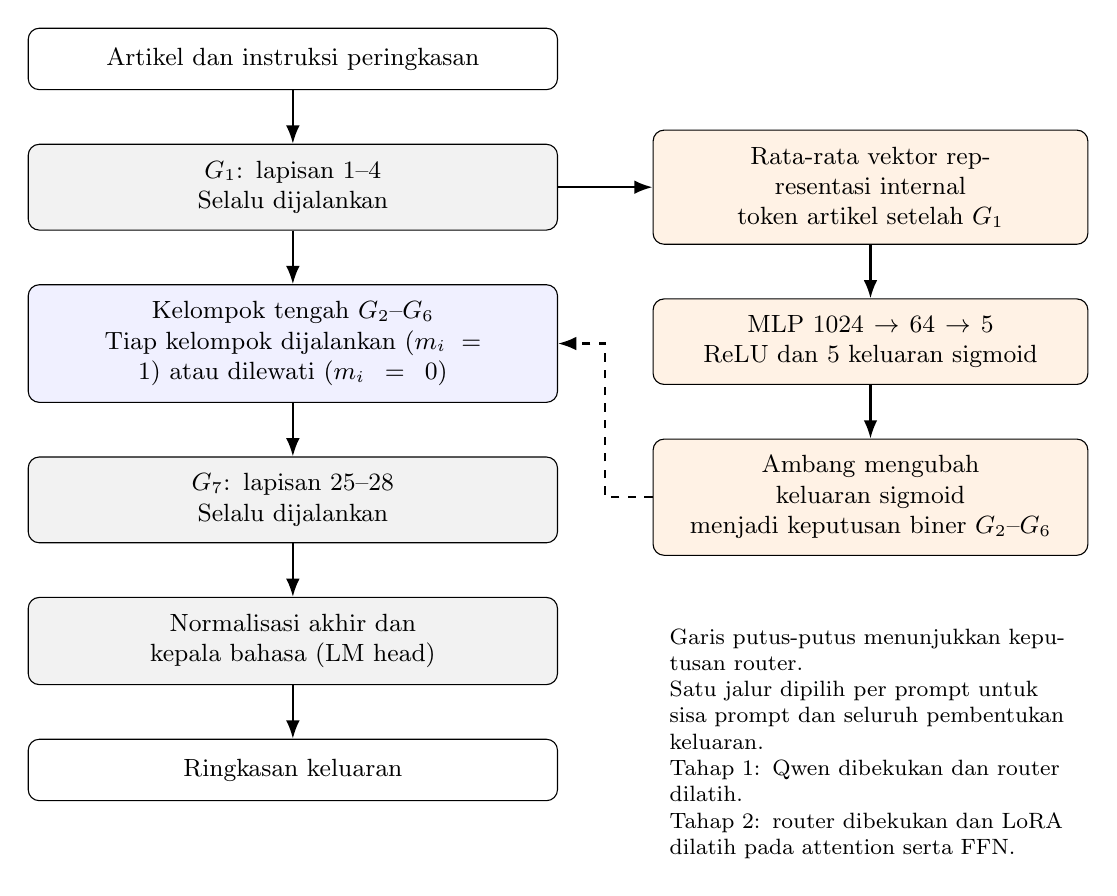
\begin{tikzpicture}[
  node distance=0.68cm and 1.2cm,
  block/.style={draw, rounded corners, align=center, text width=6.3cm,
    minimum height=0.78cm, inner sep=6pt, font=\small},
  fixed/.style={block, fill=gray!10},
  conditional/.style={block, fill=blue!6},
  router/.style={block, text width=5.1cm, fill=orange!10},
  flow/.style={-{Latex}, thick},
  control/.style={-{Latex}, dashed, thick}
]
  % Main model path
  \node[block] (input) {Artikel dan instruksi peringkasan};
  \node[fixed, below=of input] (g1) {$G_1$: lapisan 1--4\\Selalu dijalankan};
  \node[conditional, below=of g1] (middle) {Kelompok tengah $G_2$--$G_6$\\Tiap kelompok dijalankan ($m_i=1$) atau dilewati ($m_i=0$)};
  \node[fixed, below=of middle] (g7) {$G_7$: lapisan 25--28\\Selalu dijalankan};
  \node[fixed, below=of g7] (head) {Normalisasi akhir dan kepala bahasa (LM head)};
  \node[block, below=of head] (output) {Ringkasan keluaran};

  \foreach \a/\b in {input/g1,g1/middle,middle/g7,g7/head,head/output}
    \draw[flow] (\a.south) -- (\b.north);

  % Sequence-level router branch
  \node[router, right=of g1] (pool) {Rata-rata vektor representasi internal\\token artikel setelah $G_1$};
  \node[router, below=of pool] (mlp) {MLP $1024\mathbin{\to}64\mathbin{\to}5$\\ReLU dan 5 keluaran sigmoid};
  \node[router, below=of mlp] (mask) {Ambang mengubah keluaran sigmoid\\menjadi keputusan biner $G_2$--$G_6$};

  \draw[flow] (g1.east) -- (pool.west);
  \draw[flow] (pool.south) -- (mlp.north);
  \draw[flow] (mlp.south) -- (mask.north);
  \draw[control] (mask.west) -- ++(-0.6,0) |- (middle.east);

  \node[align=left, text width=5.1cm, font=\footnotesize, below=0.8cm of mask] (note)
    {Garis putus-putus menunjukkan keputusan router.\\Satu jalur dipilih per prompt untuk sisa prompt dan seluruh pembentukan keluaran.\\Tahap 1: Qwen dibekukan dan router dilatih.\\Tahap 2: router dibekukan dan LoRA dilatih pada attention serta FFN.};
\end{tikzpicture}
}
  \caption{Arsitektur konseptual sequence-level routing pada Qwen3-0.6B.}
  \label{fig:arsitektur-routing}
\end{figure}

Hasil kelompok pertama yang digunakan untuk menghitung representasi router juga dipakai untuk melanjutkan pemrosesan prompt melalui kelompok yang dipilih. Dengan demikian, kelompok pertama tidak dihitung ulang hanya untuk menjalankan router. Jalur yang dipilih dipertahankan untuk sisa pemrosesan prompt dan semua langkah pembentukan keluaran. Cache key dan value (KV cache), yaitu penyimpanan representasi yang digunakan kembali pada langkah inferensi berikutnya, disiapkan untuk lapisan yang aktif. Pada setiap token keluaran baru, kelompok pertama tetap dijalankan, tetapi router tidak memilih ulang jalur. Waktu untuk memperoleh representasi dan menjalankan router akan dimasukkan dalam waktu inferensi total. Integrasi cache dan kesetaraan perilaku dengan model penuh akan diperiksa dalam implementasi.

\subsection{Pemilihan Jalur serta Pelatihan Router dan LoRA}

Jalur adalah pola kelompok lapisan yang dijalankan untuk satu prompt. Router membuat keputusan berdasarkan prompt satu kali saja; keputusan itu tidak berubah untuk setiap token keluaran. Penelitian ini tidak menggunakan mekanisme penghentian lebih awal yang memutuskan pada setiap lapisan berdasarkan tingkat keyakinan model terhadap keluaran.

\medskip
\noindent\textbf{Kelompok Lapisan dan Keputusan Biner}\par\smallskip

Kelompok $G_1$ dan $G_7$ selalu dijalankan. Untuk tiap kelompok $G_i$, dengan $i=2,\ldots,6$, router menentukan nilai $m_i\in\{0,1\}$. Nilai satu berarti kelompok dijalankan dan nilai nol berarti kelompok dilewati. Pola lengkap ditulis sebagai $(1,m_2,m_3,m_4,m_5,m_6,1)$. Jumlah lapisan aktif tidak dipatok dan dapat berubah antarartikel dari 8 hingga 28, dengan perubahan sebanyak empat lapisan. Urutan lapisan yang dijalankan selalu mengikuti urutan Qwen.

\medskip
\noindent\textbf{Arsitektur Router dan Rencana Pelatihan}\par\smallskip

Router menggunakan jaringan perceptron multilapis (\textit{multilayer perceptron}, MLP), yaitu jaringan saraf yang memproses masukan melalui lapisan-lapisan terhubung. Masukan MLP adalah rata-rata representasi token artikel setelah $G_1$. MLP memiliki satu lapisan tersembunyi berisi 64 unit dengan fungsi aktivasi ReLU dan lima keluaran sigmoid. Setiap keluaran berpasangan dengan satu kelompok tengah. Nilai keluaran yang lebih besar atau sama dengan 0,5 diterjemahkan sebagai keputusan aktif, sedangkan nilai di bawah 0,5 diterjemahkan sebagai keputusan lewati. Saat inferensi, router hanya menerima representasi artikel dari prompt, bukan ringkasan acuannya.

Lima keputusan biner memungkinkan 32 kombinasi secara matematis. Namun, router tidak mengklasifikasikan 32 nomor jalur, dan pelatihan tidak harus menilai semua kombinasi tersebut. Pada tahap router, parameter Qwen tetap dibekukan, termasuk parameter kelompok pertama yang menghasilkan representasi router. Pada tahap berikutnya, router tetap dibekukan dan adapter LoRA dilatih pada modul attention dan FFN seluruh lapisan Qwen. Konfigurasi awal FiRST menggunakan rank 8, faktor skala 32, dan dropout 0,1; konfigurasi ini menjadi titik awal yang akan diverifikasi pada data validasi, bukan klaim konfigurasi optimal untuk Qwen3-0.6B.

Target keputusan dibuat secara luring (\textit{offline}) dari data latih. Untuk sebuah artikel dengan ringkasan acuan, setiap kandidat jalur dinilai menggunakan kerugian prediksi token dengan \textit{teacher forcing}, yaitu proses yang memberikan token acuan sebelumnya ketika menghitung prediksi token berikutnya. Skor kandidat jalur dirumuskan sebagai
\begin{equation}
  J(m) = \operatorname{NLL}(m) + \lambda C(m),
  \qquad C(m) = \frac{m_2+m_3+m_4+m_5+m_6}{5},
  \label{eq:route-objective}
\end{equation}
\noindent dengan $\operatorname{NLL}(m)$ sebagai rata-rata kerugian prediksi token pada jalur $m$, $C(m)$ sebagai proporsi kelompok tengah yang aktif, dan $\lambda$ sebagai bobot penghematan komputasi. Karena kelima kelompok memiliki jumlah lapisan yang sama, $C(m)$ digunakan sebagai ukuran sederhana proporsi kelompok yang dijalankan. Waktu inferensi aktual tetap diukur secara terpisah pada tahap evaluasi.

Pencarian target dimulai dari jalur penuh, yaitu semua kelompok tengah aktif. Pada setiap langkah, satu kelompok tengah yang masih aktif dicoba untuk dilewati. Kandidat dengan nilai $J(m)$ paling rendah dipilih jika nilainya lebih rendah daripada jalur saat ini. Proses berhenti ketika tidak ada penghapusan kelompok yang menurunkan nilai tersebut. Cara ini menghasilkan target biner untuk $G_2$ sampai $G_6$ tanpa kewajiban mengevaluasi seluruh 32 pola jalur.

Router dilatih menggunakan \textit{binary cross-entropy with logits} pada lima target biner tersebut. Penalti penghematan tidak ditambahkan ke fungsi klasifikasi karena penghematan telah digunakan saat membentuk target jalur. Konfigurasi awal router menggunakan optimizer AdamW dengan \textit{learning rate} $10^{-3}$, \textit{weight decay} $10^{-4}$, paling banyak 50 epoch, dan \textit{early stopping} dengan kesabaran lima epoch. Kandidat nilai penalti target ditetapkan sebagai $\lambda\in\{0, 0{,}01, 0{,}05, 0{,}10, 0{,}20\}$. Satu nilai $\lambda$ dipilih menggunakan data validasi dan digunakan pula saat memilih pola static. Seed pemilihan subset ditetapkan sebesar 42, sedangkan seed utama pelatihan router ditetapkan sebesar 43. Seed tambahan 44 dan 45 dapat digunakan untuk analisis ketahanan apabila sumber daya mencukupi; hasilnya akan dilaporkan terpisah dari hasil seed utama. Ringkasan acuan hanya digunakan untuk membentuk target pada pelatihan; saat inferensi, router hanya menggunakan representasi prompt. Data uji tidak digunakan untuk membentuk target atau memilih konfigurasi.

Setelah router terpilih, bobot router dibekukan dan LoRA dilatih menggunakan prompt serta ringkasan acuan dengan \textit{teacher forcing}. Adapter dipasang pada proyeksi attention dan FFN di seluruh lapisan, sedangkan bobot dasar Qwen tidak diperbarui. Konfigurasi awal FiRST menggunakan rank 8, faktor skala 32, dan dropout 0,1 \citep{jain2025first}; nilai ini menjadi titik awal, bukan klaim optimal untuk Qwen3-0.6B. Untuk metode routing adaptif, fungsi objektif LoRA menambahkan penalti non-skip berbobot $\beta$ pada probabilitas kelompok aktif, $L_{\mathrm{LoRA}}=L_{\mathrm{NLL}}+\beta\sum_{i=2}^{6}p_i$, dengan $p_i$ sebagai probabilitas router untuk menjalankan kelompok $G_i$. Penalti ini menjaga agar perubahan representasi akibat LoRA tidak menghilangkan perilaku skipping. Kandidat nilai $\beta$ serta rincian optimisasi LoRA yang belum ditetapkan dipilih atau diverifikasi menggunakan data validasi; data uji tidak digunakan untuk keputusan tersebut. Model penuh+LoRA dan static skipping+LoRA dilatih dengan konfigurasi adapter dan protokol yang sama, tanpa penalti non-skip untuk jalur yang ditetapkan tetap. Router tanpa LoRA menjadi kontrol ablation dari metode adaptif.

\subsection{Bagan Alir Metodologi}

Gambar~\ref{fig:bagan-alir-routing} merangkum urutan penelitian. Bagan membedakan persiapan yang telah tersedia dari pekerjaan implementasi dan pengujian yang masih direncanakan.

\begin{figure}[H]
  \centering
  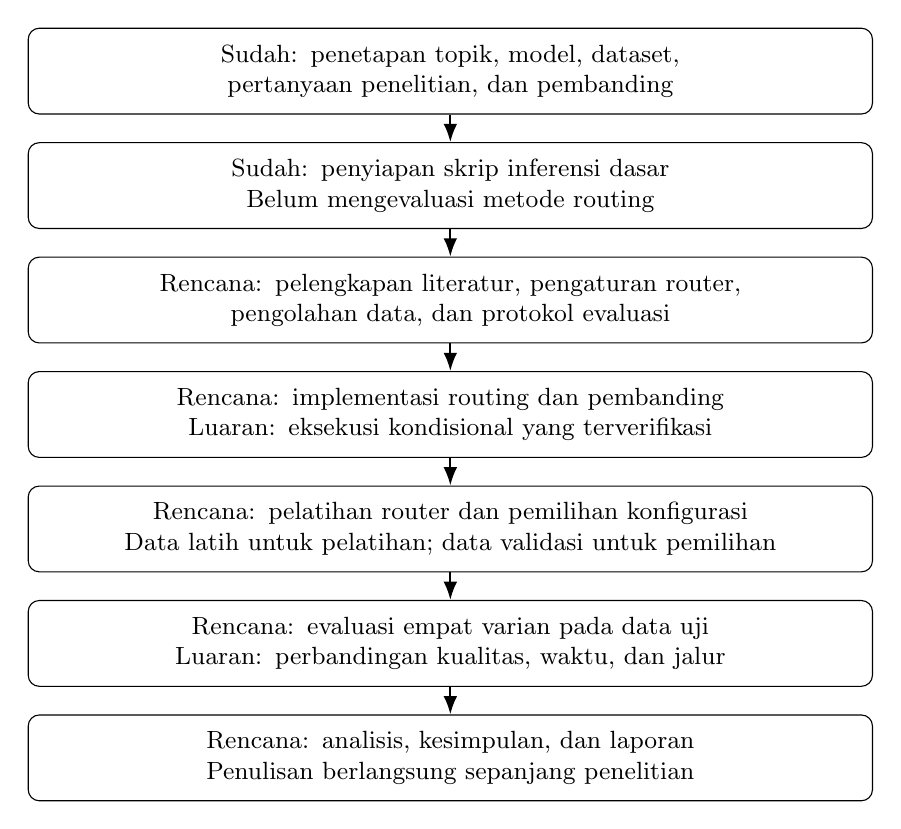
\begin{tikzpicture}[
    node distance=0.35cm,
    block/.style={draw, rounded corners, align=center, text width=10.3cm, inner sep=6pt, font=\small},
    arrow/.style={-{Latex}, thick}
  ]
    \node[block] (scope) {Sudah: penetapan topik, model, dataset,\\pertanyaan penelitian, dan pembanding};
    \node[block, below=of scope] (basic) {Sudah: penyiapan skrip inferensi dasar\\Belum mengevaluasi metode routing};
    \node[block, below=of basic] (design) {Rencana: pelengkapan literatur, pengaturan router,\\pengolahan data, dan protokol evaluasi};
    \node[block, below=of design] (implementation) {Rencana: implementasi routing dan pembanding\\Luaran: eksekusi kondisional yang terverifikasi};
    \node[block, below=of implementation] (training) {Rencana: pelatihan router dan pemilihan konfigurasi\\Data latih untuk pelatihan; data validasi untuk pemilihan};
    \node[block, below=of training] (evaluation) {Rencana: evaluasi empat varian pada data uji\\Luaran: perbandingan kualitas, waktu, dan jalur};
    \node[block, below=of evaluation] (report) {Rencana: analisis, kesimpulan, dan laporan\\Penulisan berlangsung sepanjang penelitian};
    \draw[arrow] (scope) -- (basic);
    \draw[arrow] (basic) -- (design);
    \draw[arrow] (design) -- (implementation);
    \draw[arrow] (implementation) -- (training);
    \draw[arrow] (training) -- (evaluation);
    \draw[arrow] (evaluation) -- (report);
  \end{tikzpicture}
  \caption{Bagan alir metodologi dan status pekerjaan saat draf disusun.}
  \label{fig:bagan-alir-routing}
\end{figure}

\section{Rancangan Evaluasi}

\subsection{Metode Pembanding}

Evaluasi menggunakan empat varian: model penuh+LoRA, static skipping+LoRA, router+LoRA, dan router tanpa LoRA. Model penuh+LoRA menjadi acuan kualitas dan biaya tanpa pelompatan setelah adaptasi pada tugas. Pelompatan statis menggunakan satu pola tetap yang dipilih berdasarkan data validasi. Setelah dipilih, pola tersebut digunakan untuk semua artikel, selama sisa pemrosesan prompt, dan selama seluruh pembentukan keluaran. Router+LoRA menggunakan keputusan dari representasi prompt, sedangkan kontrol router-only menggunakan bobot backbone dan router dari tahap pertama tanpa kompensasi adapter. Data uji tidak digunakan untuk memilih pola statis atau konfigurasi router maupun LoRA.

Perbandingan kualitas utama akan mencakup router+LoRA terhadap full+LoRA dan static+LoRA. Perbandingan router+LoRA dengan router-only mengukur kontribusi tahap kompensasi LoRA. Setiap kandidat pola static dengan $G_1$ dan $G_7$ aktif dinilai pada data validasi menggunakan objective $J(m)$ pada Persamaan~\ref{eq:route-objective}. Pola dengan nilai objective paling rendah dipilih dan dikunci sebelum data uji digunakan. Jika terdapat nilai yang sama, pola dengan jumlah kelompok tengah aktif lebih sedikit dipilih. Jika masih sama, digunakan urutan leksikografis menaik pada $(m_2,m_3,m_4,m_5,m_6)$ dengan nilai 0 didahulukan daripada 1. Efisiensi utama dibandingkan menggunakan waktu inferensi aktual pada lingkungan dan pengaturan yang sama, tanpa penyetaraan biaya buatan berdasarkan jumlah lapisan. Jumlah lapisan aktif dan waktu inferensi aktual akan dicatat. Jumlah lapisan yang sama belum tentu menghasilkan biaya yang sama karena waktu routing, adapter, dan panjang keluaran dapat berbeda. Jumlah lapisan aktif tidak akan digunakan sebagai pengganti pengukuran jumlah operasi aritmetika bilangan titik mengambang (\textit{floating-point operations}, FLOPs) ataupun sebagai bukti percepatan. Waktu total mencakup pekerjaan router dan adapter yang benar-benar dijalankan; metode statis tidak dibebani biaya menjalankan router yang tidak digunakan.

\subsection{Pemeriksaan Kebenaran Implementasi}

Pemeriksaan awal akan memastikan bahwa ketika semua lapisan dijalankan, implementasi memberikan perilaku yang sesuai dengan model penuh pada kondisi yang sama. Pemeriksaan juga akan memastikan bahwa lapisan yang ditandai untuk dilewati memang tidak dieksekusi, jalur tidak berubah selama pembentukan keluaran, KV cache dikelola secara konsisten, bobot router tidak berubah pada tahap LoRA, dan adapter hanya dilatih pada tahap kedua. Pemeriksaan ini dilakukan sebelum hasil kualitas dan waktu ditafsirkan.

\subsection{Kualitas Ringkasan dan Efisiensi Inferensi}

Kualitas keluaran dibandingkan dengan ringkasan acuan menggunakan ROUGE-1, ROUGE-2, dan ROUGE-L. Metrik ini mengukur kecocokan kata tunggal (unigram), pasangan kata berurutan (bigram), dan subsekuens terpanjang yang sama. Penilaian dilakukan sepenuhnya secara otomatis; tidak ada penilaian manual atau pemeriksaan faktualitas manual pada sampel. F1 akan dilaporkan untuk ROUGE-1, ROUGE-2, ROUGE-L, dan BERTScore. Untuk setiap metrik, F1 dihitung per artikel lalu dirata-ratakan secara aritmetika dengan bobot yang sama bagi setiap artikel. Keempat rata-rata dilaporkan secara terpisah. F1 tidak dihitung dari presisi dan cakupan (\textit{recall}) yang terlebih dahulu dirata-ratakan.

ROUGE akan dihitung menggunakan implementasi \texttt{rouge-score} dengan tokenisasi bawaan, tanpa stemming. Tokenisasi tersebut menormalisasi huruf menjadi huruf kecil dan memisahkan tanda baca sesuai aturan implementasi, sedangkan teks sumber dan ringkasan yang disimpan tidak diubah. Metrik yang digunakan adalah \texttt{rouge1}, \texttt{rouge2}, dan \texttt{rougeL}; \texttt{rougeL} digunakan pada tingkat kalimat, bukan \texttt{rougeLsum}. Pengaturan ini dipilih agar tidak menerapkan stemmer bahasa Inggris pada teks bahasa Indonesia. Skor F1 dikumpulkan per artikel sebelum rata-rata makro dihitung.

BERTScore melengkapi ROUGE dengan membandingkan representasi kontekstual token pada ringkasan keluaran dan ringkasan acuan menggunakan kemiripan kosinus \citep{zhang2020bertscore}. Evaluasi akan menggunakan encoder \texttt{bert-base-multilingual-cased}, parameter bahasa \texttt{id}, dan lapisan ke-9 sesuai konfigurasi standar model tersebut pada pustaka BERTScore. IDF tidak digunakan (\texttt{idf=False}) sehingga semua token diberi bobot yang sama dan skor tidak bergantung pada korpus tambahan untuk menghitung frekuensi dokumen. Skor tidak disesuaikan dengan baseline (\texttt{rescale\_with\_baseline=False}) agar konfigurasi utama tidak bergantung pada berkas baseline tambahan yang dapat berbeda menurut versi perangkat lunak. Teks untuk BERTScore hanya menggunakan pembersihan awal--akhir yang telah ditetapkan; huruf besar, tanda baca, dan isi teks lainnya dipertahankan. Jika tokenisasi encoder menghasilkan lebih dari 510 token subkata, bagian akhir teks dipotong hingga batas tersebut sebelum penilaian, dan jumlah kasus pemotongan dicatat. Konfigurasi evaluator akan sama untuk semua metode. Metrik kecocokan terhadap acuan tidak menjamin faktualitas atau kualitas ringkasan secara keseluruhan. Forde et al. menemukan bahwa metrik otomatis dapat menjadi ukuran kualitas yang tidak andal pada peringkasan multibahasa, dengan masalah yang lebih besar pada bahasa Indonesia; karena itu, hasil di sini akan ditafsirkan terbatas pada metrik yang digunakan \citep{forde2024multilingeval}.

Selisih rata-rata F1 antar-metode akan disertai interval kepercayaan dua sisi 95\% menggunakan bootstrap berpasangan. Pada setiap pengambilan ulang (\textit{resampling}), artikel diambil dengan pengembalian sebanyak jumlah artikel uji semula. Indeks artikel yang sama digunakan untuk kedua metode dalam satu perbandingan, lalu selisih rata-rata F1 dihitung ulang. Penghitungan menggunakan skor per artikel yang telah disimpan, sehingga ringkasan tidak perlu dibuat ulang. Interval menggunakan metode persentil berdasarkan 10.000 pengambilan ulang dengan seed bootstrap 42; batas bawah dan atas adalah persentil 2,5\% dan 97,5\% dari distribusi selisih. Seed bootstrap ini terpisah dari seed pemilihan subset dan pelatihan router. Interval dihitung untuk router+LoRA dibandingkan dengan full+LoRA dan static+LoRA, serta router+LoRA dibandingkan dengan router-only sebagai ablation; semua perbandingan dihitung terpisah untuk keempat metrik. Hasil utama menggunakan satu seed pelatihan router, yaitu seed 43; variasi antarseed tidak menjadi bagian dari eksperimen utama. Interval yang dihitung dari artikel mengukur variasi antarartikel dan tidak mencakup variasi antarseed.

Waktu inferensi diukur per artikel dan mencakup waktu total, waktu pemrosesan prompt (\textit{prefill}), serta waktu pembentukan keluaran (\textit{decoding}). Batas awal dan akhir pengukuran setiap komponen akan ditetapkan agar biaya representasi serta router tercakup tanpa dihitung dua kali. Jumlah token keluaran juga dicatat: waktu yang lebih singkat dapat terjadi hanya karena model menghasilkan ringkasan yang lebih pendek. Sebelum pengukuran, setiap metode dijalankan tiga kali sebagai pemanasan dan hasilnya tidak dicatat. Setelah itu, pengukuran diulang lima kali pada setiap artikel. Median dari lima pengukuran digunakan sebagai waktu utama, sedangkan variasinya dilaporkan sebagai informasi tambahan.

Semua metode akan menggunakan perangkat, presisi numerik, prompt, dan pengaturan generasi yang sama. Mode non-thinking dan greedy decoding digunakan dengan \texttt{do\_sample=False}, \texttt{num\_beams=1}, dan batas keluaran 256 token. Hasil kualitas akan dianalisis bersama biaya inferensi aktual. Frekuensi setiap pola jalur yang dipilih akan dicatat untuk mengetahui apakah router hampir selalu memilih pola yang sama. Kondisi ini disebut \textit{routing collapse}. Temuan tersebut akan dilaporkan sebagai perilaku yang diamati, bukan langsung dianggap sebagai keberhasilan atau kegagalan.

\section{Lingkungan Penelitian}

Penelitian akan dilakukan pada laptop lokal dengan CPU AMD Ryzen 3 5300U (empat inti dan delapan thread). Sistem memiliki RAM sekitar 9,1 GiB dan grafis Radeon terintegrasi. Konfigurasi penelitian menggunakan CPU, presisi FP32 (bilangan titik mengambang 32-bit), dan ukuran batch satu. Semua metode akan dievaluasi pada perangkat dan pengaturan yang sama.

Versi perangkat lunak, pengaturan thread, revisi model, dan batas token akan dicatat sebelum evaluasi. Pengukuran waktu dilakukan dengan laptop terhubung ke daya, pengaturan daya yang sama, dan aktivitas latar belakang seminimal mungkin. Kesimpulan efisiensi dibatasi pada lingkungan yang diuji.

Rancangan penelitian yang digunakan meliputi pembagian tujuh kelompok, keputusan biner untuk lima kelompok tengah, representasi prompt, arsitektur router, dua tahap pelatihan router dan LoRA, konfigurasi awal adapter, objective beserta kandidat penalti, seed pemilihan subset dan seed utama pelatihan, pemilihan pola static pada data validasi, evaluasi empat varian, perbandingan efisiensi berdasarkan waktu aktual, mode non-thinking, batas token, konfigurasi ROUGE dan BERTScore, tiga kali pemanasan, serta lima kali pengulangan pengukuran.

\chapter{JADWAL PENELITIAN}

\section{Penyusunan Jadwal}

Jadwal akan mengikuti tahapan pada Bab III: melengkapi kajian dan rancangan, menyiapkan data serta model, menerapkan eksekusi kondisional, melatih router, mengevaluasi hasil, dan menulis laporan. Dokumentasi serta penulisan proposal akan dilakukan seiring pekerjaan teknis.

Waktu mulai, durasi penelitian, alokasi waktu untuk setiap kegiatan, dan ketersediaan perangkat komputasi belum ditetapkan. Karena itu, bagan Gantt yang menunjukkan kegiatan per bulan akan dilengkapi setelah jadwal disepakati. Uraian ini belum menetapkan tanggal atau komitmen durasi penelitian.


%------------------------------------------------------------
% Bibliography
%------------------------------------------------------------
\bibliography{references}

\end{document}
